% Notes de cours pour ACT-2005
% Automne 2018
\documentclass[12pt, french]{report}

% Lien vers un template de préambule
% !TEX encoding = UTF-8 Unicode
% LaTeX Preamble
% Author : Gabriel Crépeault-Cauchon
% Last update : 07/10/2018

% HOW-TO : copy-paste this file in the same directory as your .tex file, and add in your preamble the next command right after you have specified your documentclass : 
% % !TEX encoding = UTF-8 Unicode
% LaTeX Preamble
% Author : Gabriel Crépeault-Cauchon
% Last update : 07/10/2018

% HOW-TO : copy-paste this file in the same directory as your .tex file, and add in your preamble the next command right after you have specified your documentclass : 
% % !TEX encoding = UTF-8 Unicode
% LaTeX Preamble
% Author : Gabriel Crépeault-Cauchon
% Last update : 07/10/2018

% HOW-TO : copy-paste this file in the same directory as your .tex file, and add in your preamble the next command right after you have specified your documentclass : 
% \input{preambule_utf8.tex}

% ---------------------------------------------
% BEGINNING OF PREAMBLE
% ---------------------------------------------
% Encoding packages
\usepackage[utf8]{inputenc}
\usepackage[T1]{fontenc}
\usepackage{babel}
\usepackage{lmodern}

% HYPERREF (URL's and Link options)
\usepackage{hyperref}
\hypersetup{colorlinks = true, urlcolor = blue, linkcolor = red!60!black}

% POLICY (choose one of them)
%	\usepackage{concrete}
%	\usepackage{mathpazo}
%	\usepackage{frcursive} %% permet d'écrire en lettres attachées
 \usepackage{aeguill}
% 	\usepackage{mathptmx}
%	\usepackage{fourier} 

% Mathematics configuration
\usepackage{amsmath,amsthm,amssymb,latexsym,amsfonts}
\usepackage{empheq}
\usepackage{numprint}
\usepackage{dsfont} 


% Tcolorbox config
\usepackage{tcolorbox}
\tcbuselibrary{xparse}
\tcbuselibrary{breakable}
%% Définition Boite pour exemple
\newcounter{ex}[section]
\DeclareTColorBox{exemple}{ o }% #1 parameter
{colframe=green!20!black,colback=green!5!white, % color of the box
breakable, pad at break*=0mm, % to split the box
before title = {\textbf{Exemple \stepcounter{ex} \arabic{chapter}.\arabic{section}.\arabic{ex} }},
IfValueTF = {#1}{title= {#1}}{title= \hphantom},
after title = {\large \hfill \faWrench}
}

%% Définition boite pour définition
\newcounter{def}[section]
\DeclareTColorBox{definition}{ o }% #1 parameter
{colframe=blue!60!green,colback=blue!5!white, % color of the box
breakable, pad at break*=0mm, % to split the box
before title = {\textbf{Définition \stepcounter{def} \arabic{chapter}.\arabic{section}.\arabic{def} }},
title = {#1},
after title = {\large \hfill \faBook}
}


% Graphics and picture import Packages
\usepackage{graphicx}
\usepackage{pict2e}

% insert PDF package
\usepackage{pdfpages}

% Color package
\usepackage{color, soulutf8, colortbl}

% usefull shortcut for colored text
\newcommand{\orange}{\textcolor{orange}}
\newcommand{\red}{\textcolor{red}}
\newcommand{\cyan}{\textcolor{cyan}}
\newcommand{\blue}{\textcolor{blue}}
\newcommand{\green}{\textcolor{green}}
\newcommand{\purple}{\textcolor{magenta}}
\newcommand{\yellow}{\textcolor{yellow}}

% Custum enumerate & itemize Package
\usepackage{enumitem}
% French Setup for itemize function
\frenchbsetup{StandardItemLabels=true}

% Mathematics shortcut
\usepackage{cancel}
\newcommand{\reels}{\mathbb{R}}
\newcommand{\entiers}{\mathbb{Z}}
\newcommand{\naturels}{\mathbb{N}}
\newcommand{\eval}{\biggr \rvert}
\newcommand{\esp}[1]{\mathrm{E} \left[ #1 \right]} % espérance
\newcommand{\variance}[1]{\mathrm{Var} \left( #1 \right)} % variance
\newcommand{\covar}[1]{\mathrm{Cov} \left( #1 \right)} % variance
\newcommand{\prob}[1]{\Pr \left( #1 \right)} % probabilité entre parenthèses
\newcommand{\laplace}{\mathcal{L}}

% Actuarial notation package
\usepackage{actuarialsymbol}
\usepackage{actuarialangle}

% To indicate equation number on a specific line in align environment
\newcommand\numberthis{\addtocounter{equation}{1}\tag{\theequation}}

% Other shortcut
\newcommand{\p}{\paragraph{}}
\newcommand{\n}{\newline}
\newcommand{\derivee}[1]{\frac{\partial}{\partial #1}}
\newcommand{\indic}[1]{\mathds{1}_{\{ #1 \}}}

% Special symbols package
\usepackage[tikz]{bclogo}
\usepackage{fontawesome}

% Retire l'indentation automatique de Latex
\setlength{\parindent}{0pt}

% ---------------------------------------------
% END OF PREAMBLE
% ---------------------------------------------

% ---------------------------------------------
% BEGINNING OF PREAMBLE
% ---------------------------------------------
% Encoding packages
\usepackage[utf8]{inputenc}
\usepackage[T1]{fontenc}
\usepackage{babel}
\usepackage{lmodern}

% HYPERREF (URL's and Link options)
\usepackage{hyperref}
\hypersetup{colorlinks = true, urlcolor = blue, linkcolor = red!60!black}

% POLICY (choose one of them)
%	\usepackage{concrete}
%	\usepackage{mathpazo}
%	\usepackage{frcursive} %% permet d'écrire en lettres attachées
 \usepackage{aeguill}
% 	\usepackage{mathptmx}
%	\usepackage{fourier} 

% Mathematics configuration
\usepackage{amsmath,amsthm,amssymb,latexsym,amsfonts}
\usepackage{empheq}
\usepackage{numprint}
\usepackage{dsfont} 


% Tcolorbox config
\usepackage{tcolorbox}
\tcbuselibrary{xparse}
\tcbuselibrary{breakable}
%% Définition Boite pour exemple
\newcounter{ex}[section]
\DeclareTColorBox{exemple}{ o }% #1 parameter
{colframe=green!20!black,colback=green!5!white, % color of the box
breakable, pad at break*=0mm, % to split the box
before title = {\textbf{Exemple \stepcounter{ex} \arabic{chapter}.\arabic{section}.\arabic{ex} }},
IfValueTF = {#1}{title= {#1}}{title= \hphantom},
after title = {\large \hfill \faWrench}
}

%% Définition boite pour définition
\newcounter{def}[section]
\DeclareTColorBox{definition}{ o }% #1 parameter
{colframe=blue!60!green,colback=blue!5!white, % color of the box
breakable, pad at break*=0mm, % to split the box
before title = {\textbf{Définition \stepcounter{def} \arabic{chapter}.\arabic{section}.\arabic{def} }},
title = {#1},
after title = {\large \hfill \faBook}
}


% Graphics and picture import Packages
\usepackage{graphicx}
\usepackage{pict2e}

% insert PDF package
\usepackage{pdfpages}

% Color package
\usepackage{color, soulutf8, colortbl}

% usefull shortcut for colored text
\newcommand{\orange}{\textcolor{orange}}
\newcommand{\red}{\textcolor{red}}
\newcommand{\cyan}{\textcolor{cyan}}
\newcommand{\blue}{\textcolor{blue}}
\newcommand{\green}{\textcolor{green}}
\newcommand{\purple}{\textcolor{magenta}}
\newcommand{\yellow}{\textcolor{yellow}}

% Custum enumerate & itemize Package
\usepackage{enumitem}
% French Setup for itemize function
\frenchbsetup{StandardItemLabels=true}

% Mathematics shortcut
\usepackage{cancel}
\newcommand{\reels}{\mathbb{R}}
\newcommand{\entiers}{\mathbb{Z}}
\newcommand{\naturels}{\mathbb{N}}
\newcommand{\eval}{\biggr \rvert}
\newcommand{\esp}[1]{\mathrm{E} \left[ #1 \right]} % espérance
\newcommand{\variance}[1]{\mathrm{Var} \left( #1 \right)} % variance
\newcommand{\covar}[1]{\mathrm{Cov} \left( #1 \right)} % variance
\newcommand{\prob}[1]{\Pr \left( #1 \right)} % probabilité entre parenthèses
\newcommand{\laplace}{\mathcal{L}}

% Actuarial notation package
\usepackage{actuarialsymbol}
\usepackage{actuarialangle}

% To indicate equation number on a specific line in align environment
\newcommand\numberthis{\addtocounter{equation}{1}\tag{\theequation}}

% Other shortcut
\newcommand{\p}{\paragraph{}}
\newcommand{\n}{\newline}
\newcommand{\derivee}[1]{\frac{\partial}{\partial #1}}
\newcommand{\indic}[1]{\mathds{1}_{\{ #1 \}}}

% Special symbols package
\usepackage[tikz]{bclogo}
\usepackage{fontawesome}

% Retire l'indentation automatique de Latex
\setlength{\parindent}{0pt}

% ---------------------------------------------
% END OF PREAMBLE
% ---------------------------------------------

% ---------------------------------------------
% BEGINNING OF PREAMBLE
% ---------------------------------------------
% Encoding packages
\usepackage[utf8]{inputenc}
\usepackage[T1]{fontenc}
\usepackage{babel}
\usepackage{lmodern}

% HYPERREF (URL's and Link options)
\usepackage{hyperref}
\hypersetup{colorlinks = true, urlcolor = blue, linkcolor = red!60!black}

% POLICY (choose one of them)
%	\usepackage{concrete}
%	\usepackage{mathpazo}
%	\usepackage{frcursive} %% permet d'écrire en lettres attachées
 \usepackage{aeguill}
% 	\usepackage{mathptmx}
%	\usepackage{fourier} 

% Mathematics configuration
\usepackage{amsmath,amsthm,amssymb,latexsym,amsfonts}
\usepackage{empheq}
\usepackage{numprint}
\usepackage{dsfont} 


% Tcolorbox config
\usepackage{tcolorbox}
\tcbuselibrary{xparse}
\tcbuselibrary{breakable}
%% Définition Boite pour exemple
\newcounter{ex}[section]
\DeclareTColorBox{exemple}{ o }% #1 parameter
{colframe=green!20!black,colback=green!5!white, % color of the box
breakable, pad at break*=0mm, % to split the box
before title = {\textbf{Exemple \stepcounter{ex} \arabic{chapter}.\arabic{section}.\arabic{ex} }},
IfValueTF = {#1}{title= {#1}}{title= \hphantom},
after title = {\large \hfill \faWrench}
}

%% Définition boite pour définition
\newcounter{def}[section]
\DeclareTColorBox{definition}{ o }% #1 parameter
{colframe=blue!60!green,colback=blue!5!white, % color of the box
breakable, pad at break*=0mm, % to split the box
before title = {\textbf{Définition \stepcounter{def} \arabic{chapter}.\arabic{section}.\arabic{def} }},
title = {#1},
after title = {\large \hfill \faBook}
}


% Graphics and picture import Packages
\usepackage{graphicx}
\usepackage{pict2e}

% insert PDF package
\usepackage{pdfpages}

% Color package
\usepackage{color, soulutf8, colortbl}

% usefull shortcut for colored text
\newcommand{\orange}{\textcolor{orange}}
\newcommand{\red}{\textcolor{red}}
\newcommand{\cyan}{\textcolor{cyan}}
\newcommand{\blue}{\textcolor{blue}}
\newcommand{\green}{\textcolor{green}}
\newcommand{\purple}{\textcolor{magenta}}
\newcommand{\yellow}{\textcolor{yellow}}

% Custum enumerate & itemize Package
\usepackage{enumitem}
% French Setup for itemize function
\frenchbsetup{StandardItemLabels=true}

% Mathematics shortcut
\usepackage{cancel}
\newcommand{\reels}{\mathbb{R}}
\newcommand{\entiers}{\mathbb{Z}}
\newcommand{\naturels}{\mathbb{N}}
\newcommand{\eval}{\biggr \rvert}
\newcommand{\esp}[1]{\mathrm{E} \left[ #1 \right]} % espérance
\newcommand{\variance}[1]{\mathrm{Var} \left( #1 \right)} % variance
\newcommand{\covar}[1]{\mathrm{Cov} \left( #1 \right)} % variance
\newcommand{\prob}[1]{\Pr \left( #1 \right)} % probabilité entre parenthèses
\newcommand{\laplace}{\mathcal{L}}

% Actuarial notation package
\usepackage{actuarialsymbol}
\usepackage{actuarialangle}

% To indicate equation number on a specific line in align environment
\newcommand\numberthis{\addtocounter{equation}{1}\tag{\theequation}}

% Other shortcut
\newcommand{\p}{\paragraph{}}
\newcommand{\n}{\newline}
\newcommand{\derivee}[1]{\frac{\partial}{\partial #1}}
\newcommand{\indic}[1]{\mathds{1}_{\{ #1 \}}}

% Special symbols package
\usepackage[tikz]{bclogo}
\usepackage{fontawesome}

% Retire l'indentation automatique de Latex
\setlength{\parindent}{0pt}

% ---------------------------------------------
% END OF PREAMBLE
% ---------------------------------------------
% % Preamble for code listing
% Please input this file after your main preamble
% Gabriel Crépeault-Cauchon, 2018
% -------------------------------

% Load the package 
\usepackage{listings}

% -------
% Settings for different programming language : 

% VISUAL BASIC FOR APPLICATION (VBA)
\lstdefinestyle{vba}
{
	language = {[Visual] Basic},	
	breaklines = true,
	extendedchars=\true,
	showstringspaces = false,	
	tabsize = 3,
	breaklines = true,
	keywordstyle = \color{blue},
	commentstyle = \color{green!35!black},
	backgroundcolor = \color{gray!20!white},
	stringstyle = \color{red}
}


% R (to be modified : does not work for now.
\lstdefinestyle{SAS}
{
	language=SAS
}




% Information sur le document
\title{Mathématiques actuarielles IARD-1 \\
ACT-2005 \\
Notes de cours}
\author{Gabriel Crépeault-Cauchon \\
Nicholas Langevin}


% -----------------------------------
% --- DÉBUT DU DOCUMENT ---
\begin{document}

% Page titre
\maketitle

% Table des matières
\tableofcontents

% --- DÉBUT DE LA RÉDACTION ---

% --- RÉSUMÉ ---
\begin{abstract}
Ce document résume les notes de cours prises en classe dans le cours de Mathématiques actuarielles IARD-1, ainsi que des notions prises du livre \textit{LOSS MODELS - From Data to Decisions, 4\up{th} edition}.
\end{abstract}
% --------------

\chapter{Rappel sur les notions de probabilité et statistiques}
\section{Quantités à savoir}

\paragraph{\textit{Raw moments}}
On représente le $k$\up{e} moment par $\mu_k^\prime$, soit
\begin{equation}
\mu_k^\prime = \esp{X^k} 
\end{equation}

\paragraph{Moments centraux} Le $k$\up{e} moment central est représenté par
\begin{equation}
\mu_k = \esp{(X - \mu)^k}
\end{equation}

\begin{exemple}[Quelques exemples de moments centraux]
La variance est le 2\up{e} moment central : 
\begin{align*}
Var(X) = \mu_2 =  \esp{(X - \mu)^2} \\
\end{align*}
Le 3\up{e} moment centré, qui est utilisé pour calculer le coefficient d'asymétrie : 
\begin{align*}
\mu_3 = \esp{(X-\mu)^3}
\end{align*}
\end{exemple}

\paragraph{Coefficient d'asymétrie}
Le coefficient d'asymétrie, aussi appelé \textit{skewness}, est représentée par
\begin{equation}
S_k = \frac{\mu_3}{\sigma^2}
\end{equation}
Soit le 3\up{e} moment standarisé. Si $S_k = 0$, alors la distribution tend vers une loi normale.

\paragraph{Coefficient d'applatissement}
Le coefficient d'applatissement, aussi appelé \textit{Kurtosis}, se définit par
\begin{equation}
\text{Kurtosis} = \frac{\mu_4}{\sigma^4}
\end{equation}
Cette quantité permet de mesurer l'épaisseur de l'aile (\textit{tail}) de la distribution. Si $\esp{z^4} =3$, alors la distribution tend vers une loi normale $N(\mu, \sigma^2)$.

\section{La loi normale}

\paragraph{La fonction génératrice des moments}
\begin{align*}
    M_x(t) &= M_x(0) + \frac{M_x^\prime t}{1!} + \frac{M_x^{\prime\prime} t^2}{2!} + ... + \frac{M_x^{(n) t^n}}{n!} \\
           &= 1 + \frac{E[x] t}{1!} + \frac{E[x^2] t^2}{2!} + ... + \frac{E[x^n] t^n}{n!}
\end{align*}

On pose: $c_k = \frac{E[x^n]}{n!}$ alors,

\begin{equation}
    E[x^k] = C_k k!
\end{equation}

\section{Queue de distribution}

\begin{enumerate}
    \item Sois $f_1(x)$ une fonction tels que les 3 premiers moment existe: $E[x^4] = \infty$
    \item Sois $f_2(x)$ une fonction tels que les 2 premiers moment existe: $E[x^2] = \infty$
\end{enumerate}
Alors,
\begin{align*}
    \lim_{x\to\infty} r(x) = \frac{f_1(x)}{f_2(x)} = \left\{
                                                        \begin{array}{ll}
                                                            \infty ,\: f_1(x) \text{a une aile plus lourde que} f_2(x) \\
                                                            0      ,\: f_2(x) \text{a une aile plus lourde que} f_1(x) 
                                                        \end{array}
                                                    \right.
\end{align*}
\begin{exemple}
    Sois $f_{x_1}(x_1) \sim pareto(\alpha, \theta)$ et $f_{x_2}(x_2) \sim gamma(\alpha, \lambda)$ 
    \begin{align*}
        \lim_{x\to\infty} r(x) &= \lim_{x\to\infty} \frac{f_{x_1}(x_1)}{f_{x_2}(x_2)} \\
                               &= \frac{\frac{\alpha \theta^\alpha}{(x + \theta)^{\alpha + 1}}}{\lambda^\alpha x^{\alpha - 1} e^{-\lambda x}} \\
                               &= C \frac{e^{-\lambda x}}{x^{\alpha - 1} (x + \theta)^{\alpha + 1}} \\
                               &= \infty
    \end{align*}      
    La pareto a une queue plus lourde que la gamma
\end{exemple}

\paragraph{La fonction de hasard}
\begin{equation}
    h(x) = \frac{f(x)}{s(x)}
\end{equation}
Si à partir de M, $h(x)$ est décroissante $\Leftrightarrow$ $f(x)$ décroit trop lentement, alors $f(x)$ à une aile lourde. 




\chapter{Types de contrats et primes}
Dans cette section \footnote{Section 8.1 à 8.5 dans le livre}, on définit deux nouvelles variables
\begin{definition}[\textit{Per-Loss} Variable]
Soit $X$ le montant des dommages d'une réclamation. On peut définir $Y^L$ comme le montant payé par l'assureur lors de toute perte. Mathématiquement,
\begin{equation}
Y^L = g(X) \quad , Y^L \sim f_X(x)
\end{equation}
\end{definition}

\begin{definition}[\textit{Per-Payment} variable]
Cette variable se définit plutôt comme le montant qui sera payé par l'assureur (i.e le montant de la perte, sachant qu'il y aura un paiement). Alors,
\begin{equation}
Y^P = g(X) \quad , Y^P \sim \frac{f_X(x)}{S_X(x)}
\end{equation}
$Y^P$ n'a donc pas de probabilité définie à $y=0$ (puisque ce n'est pas possible, sachant que $x$ est assez grand pour qu'il y ait un paiement.
\end{definition}



\section{Contrat avec limite}
\label{sec:limite-sans-inflation}
On analyse la fonction de perte d'un contrat avec une limite supérieure $u$. Alors, on définit $Y$ comme


\begin{equation}
Y	 = (X \wedge u) = \min(X, u) = \begin{cases}
x	& , x \leq u \\
u	& , x > u \\
\end{cases}
\end{equation}

Aussi,
\begin{align*}
\esp{Y}	& = \esp{\min(X,u)} \\
	& = \int_{0}^{u} x f_X(x) dx + u \int_{u}^{\infty} f_X(x) dx \\
	& = \int_{0}^{u} x f_X(x) dx + u S(u) \\
\end{align*}



\subsection{Cas avec inflation}
On a vu le contrat avec perte limitée, mais sans parler d'inflation. Supposons qu'on a le scénario \underline{avec inflation}, où $X' = (1+r)X$ et $r$ représente le taux d'inflation appliqué au montant de perte. Alors, il faut ajuster $u$ pour tenir compte de l'inflation.

\begin{align*}
Y & = 
\begin{cases}
(1+r) X	&, (1+r)X \leq u \\
u		&, (1+r) X > u \\
\end{cases} \\
	& = 
\begin{cases}
(1+r)X	&, x \leq \frac{u}{1+r} \\
u		&, x > \frac{u}{1+r} \\
\end{cases} \\
\end{align*}
\begin{definition}[Prime Limited Loss sous l'inflation]
\begin{equation}
\esp{X' \wedge u} = (1+r) \esp{X  \wedge \frac{u}{1+r}} 
\end{equation}
\end{definition}

\begin{proof}
\begin{align*}
\esp{Y}	& = \int_{0}^{\frac{u}{1+r}} (1+r) x f_X(x) dx  + u \int_{\frac{u}{1+r}}^{\infty} f_X(x) dx \\
	& = (1+r) \int_{0}^{\frac{d}{1+r}} f f_X(x) dx + s S_X \left( \frac{u}{1+r} \right) \\
	& = (1+r) \left( \int_{0}^{\frac{u}{1+r}} x f_X(x) dx  + \frac{u}{1+r} S_X \left( \frac{u}{1+r} \right)    \right)	 \\
	& = (1+r) \esp{X  \wedge \frac{u}{1+r}}  \\
\end{align*}
\end{proof}





\section{Contrat avec déductible ordinaire}
Soit un contrat avec perte $X$, où on paie 0 si $X \leq d$ et $X-d$ si $X > d$, où $d$ est le déductible ordinaire. Alors,

\begin{equation}
Y = (X-d)_+ = \max(X-d,0) = 
\begin{cases}
0		& , X \leq d \\
X - d	& , X > d \\
\end{cases}
\end{equation}



\subsection{Remarques}

\begin{enumerate}[label=(\arabic*)]
\item $X$ est une variable aléatoire continue

\item mais $Y^L$ est une variable aléatoire mixte, car
\begin{align*}
\prob{Y^L = y} & = 
\begin{cases}
F_X(d)	& ,y = 0 \\
f_X(y+d)	& , y > 0 \\
\end{cases}
\end{align*}


\item La fonction de répartition de $Y^L$ est définie par
\begin{align*}
F_Y(y)	& = 
\begin{cases}
F_X(d)	& , y = 0 \\
F_X(d) + \int_{0}^{y} f_X(u+d) du \\
\cancel{F_X(d)} + F_X(y+d) \cancel{- F_X(d)} \\
F_X(y + d)	& y > 0 \\
\end{cases}
\end{align*}
\item les fonctions de survie $S(y)$ et fonction de hasard $h(y)$ sont définies par
\begin{align*}
S_Y(y) 	& = 1 - F_Y(y) \\
h(y)		& = \frac{f_Y(y)}{S_Y(y)} \\
\end{align*}

\item La prime de ce contrat est appelée la prime \textit{stop-loss}, qui représente l'espérance de ce contrat.
\end{enumerate}

\subsection{Prime Stop-Loss}
On veut calculer l'espérance du contrat avec déductible ordinaire : 
\begin{align*}
E[Y]		& = \esp{(X-d)_+} \\
	& = \int_{d}^{\infty} (x-d) f(x) dx \\
	& = \underbrace{\int_{d}^{\infty} x f(x) dx}_{\text{Intégration par partie}} - d \int_{d}^{\infty} f(x) dx \\
	& = -x S(x) \eval_d^\infty + \int_{d}^{\infty} S(x) dx  - s S(d) \\
	& = 0  \cancel{+ S(d)} +  \int_{d}^{\infty} S(x) dx  \cancel{- S(d)} \\
	& = \int_{d}^{\infty} S(x) dx \\
\end{align*}

\begin{definition}[Prime Stop-Loss]
On peut définir la prime Stop-Loss comme
\begin{equation}
\esp{(X-d)_+} = \esp{X} - \esp{X \wedge d}
\end{equation}
\begin{proof}
% Intégrer la preuve faite en dépannage le 20 septembre par Marianne avec les intégrales.
À compléter
\end{proof}
\end{definition}

\subsection{Cas avec inflation}
\begin{align*}
Y	& = 
\begin{cases}
0		&, X' \leq d \\
X' - d	&, d' > d \\
\end{cases}
\end{align*}
où $X' = (1+r)X$. On peut travailler seulement avec le $X$ initial : 
\begin{align*}
Y	& = 
\begin{cases}
0			&, x \leq \frac{d}{1+r} \\
(1+r)X - d 	&, x > \frac{d}{1+r} \\
\end{cases}
\end{align*}

Et la prime \textit{Stop-Loss},
\begin{align*}
\esp{Y}		& = \int_{\frac{d}{1+r}}^{\infty} ((1+r) x - d) f_X(x) dx \\
			& = (1+r) \int_{\frac{d}{1+r}}^{\infty} x f_X(x) dx - \frac{d}{1+r} \int_{\frac{d}{1+r}}^{\infty} f_X(x) dx \\
\end{align*}

\begin{definition}[Prime Stop-Loss sous le scénario d'inflation]
\begin{equation}
\esp{(X'-d)_+} = (1+r) \left( \esp{X} - \esp{X \wedge \frac{d}{1+r}} \right)
\end{equation}
\end{definition}
\begin{proof}
\begin{align*}
\esp{Y}	& = (1+r) \int_{\frac{d}{1+r}}^{\infty} x f_X(x) dx - d \int_{\frac{d}{1+r}}^{\infty} f_X(x) dx \\
	\shortintertext{En ajoutant un terme,} \\
	& = \underbrace{(1+r) \blue{\int_{0}^{\frac{d}{1+r}} x f_X(x) dx} + \int_{\frac{d}{1+r}}^{\infty} x f_X(x) dx}_{\esp{X}} - \underbrace{\blue{ \int_{0}^{\frac{d}{1+r}} x f_X(x) dx} - \frac{d}{1+r} \int_{\frac{d}{1+r}}^{\infty} f_X(x) dx}_{\esp{X \wedge \frac{d}{1+r}}} \\ 
	& = \esp{X} - \esp{X \wedge \frac{d}{1+r}} \\
\end{align*}
\end{proof}


\section{Mean Excess Loss}
Le Mean Excess Loss représente la perte excédentaire à $d$, sachant que $X > d$. Mathématiquement,
\begin{align*}
Y & = 
\begin{cases}
0		& , x \leq d \\
X - d 	& , x > d \\
\end{cases}
\end{align*}
où $X \sim \frac{f(x)}{S(d)}, x \geq d$.

\subsection{Remarques}
\begin{enumerate}[label=(\arabic*)]
\item La fonction de densité de $Y$ est représentée par
\begin{align*}
\prob{Y^P = y} & =
\begin{cases}
\frac{f_X(y+d)}{S(d)} &  , y > 0 \\
\end{cases} 
\end{align*}

\item $Y$ est une v.a. continue

\item les fonctions de survie et de hasard sont, respectivement  :
\begin{align*}
h(y)	 	& = \frac{f_Y(y_d)}{S_Y(y+d)} \\
S(y)		& = \frac{S_X(y+d)}{S(d)} \\
\end{align*}

\item l'espérance de la v.a. $Y^P$\footnote{Le $P$ en exposant signifie \textit{per pay}, qui indique que $Y$ est conditionnée sur $X$.} (mean excess loss) est définie par
\begin{align*}
e(d) & = \esp{Y^P} \\
	& =  \esp{X - d | X > d} \\
	& = \int_{d}^{\infty} (x-d) \frac{f(x)}{S(d)} dx \\
\end{align*}
On note donc
\begin{equation}
e(d) S(d)	= \underbrace{\int_{d}^{\infty} (x-d) f(x) dx}_{\text{Prime Stop-Loss}}
\end{equation}
\end{enumerate}

\begin{definition}[Loss Eliminating Ratio]
Le Loss Eliminating Ratio ($LER$), nous permet d'obtenir le pourcentage de perte qu'on ne paiera pas grâce au déductible $d$ : 
\begin{align*}
ELR 	& = \frac{\esp{X} - \esp{(X-d)_+}}{\esp{X}} \\
\shortintertext{Mais on sait que}
\esp{(X-d)_+}	& = \esp{X} - \esp{X \wedge d} \\
\end{align*}
Alors,

\begin{equation}
ELR  = \frac{\esp{X \wedge d}}{\esp{X}} 
\end{equation}
\end{definition}

\section{Contrat avec Déductible franchise}
Soit $Y$ le contrat qui a un déductible franchise. Dans ce type de contrat, on va payer l'intégralité de la perte, lorsque celle-ci dépassera un déductible. Mathématiquement,
\begin{align*}
Y	& = 
\begin{cases}
0	& , X \leq d \\
X	& , X > d \\
\end{cases}
\end{align*}

\subsubsection{Caractéristiques}
\begin{enumerate}[label=(\arabic*)]
\item La fonction de densité est définie par
\begin{align*}
f_Y(y)	& = 
\begin{cases}
F_X(d)	&, y = 0 \\
f_X(y)	&, y > 0 \\
\end{cases}
\end{align*}


\item La fonction de répartition de ce contrat est
\begin{align*}
F_Y(y)	& = 
\begin{cases}
F_X(d)	& , y = 0 \\
F_X(d)	& , 0 < y \leq d \\
\frac{F_X(y) - F_X(d)}{S_X(d)}	& , y > d \\
\end{cases}
\end{align*}
\end{enumerate}


\section{Contrat avec déductible ordinaire et limite sous l'inflation}
On peut combiner les contrats vu plus tôt, comme c'est le cas ici : ce contrat prévoit un déductible ordinaire $d$ ainsi qu'une limite au contrat $u$. De plus, on s'intéresse au scénario sous l'inflation.Alors,
\begin{align*}
Y & = 
\begin{cases}
0				& , X \leq \frac{d}{1+r} \\
(1+r) X - d		& , \frac{d}{1+r} \leq X \leq \frac{u}{1+r} \\
u=d				& , X > \frac{u}{1+r} \\
\end{cases}
\end{align*}
Et l'espérance est
\begin{definition}[Prime d'un contrat avec déductible $d$ et limite $u$]
\begin{equation}
\label{eq:prime-contrat-deductible+limite}
\esp{Y} = (1+r) \left( \esp{X \wedge \frac{u}{1+r}} - \esp{X \wedge \frac{d}{1+r}}   \right)
\end{equation}
\end{definition}

\begin{proof}
On va utiliser $Y = Y_1 - Y_2$ pour prouver \eqref{eq:prime-contrat-deductible+limite}. On définit $Y_1$ et $Y_2$ : 
\begin{align*}
Y_1	& = 
\begin{cases}
0				& , X \leq \frac{d}{1+r} \\
(1+r)X - d		& , X  > \frac{d}{1+r} \\
\end{cases} \\
Y_2	& = 
\begin{cases}
0				& , X \leq \frac{u}{1+r} \\
(1+r) X - u		& , X > \frac{u}{1+r} \\
\end{cases} \\
\shortintertext{On connait leur espérance respective,} \\
\esp{Y_1}	& = (1+r) \left( \esp{X} - \esp{X \wedge \frac{d}{1+r}} \right) \\
\esp{Y_2}	& = (1+r) \left(\esp{X} - \esp{X \wedge \frac{u}{1+r}} \right) \\
\shortintertext{Alors,}
\esp{Y}		& = \esp{Y_1} - \esp{Y_2} \\
			& = (1+r) \left( \esp{X \wedge \frac{u}{1+r}} - \esp{X \wedge \frac{d}{1+r}}  \right) \\
\end{align*}
\end{proof}

\begin{align*}
\esp{Y}	& = \int_{\frac{d}{1+r}}^{\frac{u}{1+r}} ((1+r) x - d) f_X(x) dx + \int_{\frac{u}{1+r}}^{\infty} (u-d) f_X(x) dx \\
	& = (1+r) \left( \esp{X \wedge \frac{u}{1+r}} - \esp{X \wedge \frac{d}{1+r}}   \right) \\
\end{align*}


\section{Co-assurance}
Soit $\alpha$ le pourcentage de co-assurance.

\begin{align*}
Y	& = 
\begin{cases}
0		& , X \leq d \\
X - d	& , X > d \\
\end{cases}
\end{align*}

\begin{align*}
Y^C	& = 
\begin{cases}
0		& , X  \leq d \\
\alpha(X - d) 	& , X > d \\
\end{cases}
\end{align*}
Alors,
\begin{equation}
\esp{Y^C} = \alpha \esp{Y}
\end{equation}

\section{Cas général}
Voici une formule générale, avec un déductible $d$, un taux d'inflation $r$, un pourcentage de coassurance de $\alpha$ et une limite de $u$ : 
\begin{equation}
Y^L = 
\begin{cases}
0		& ,\ x \leq \frac{d}{1+r} \\
\alpha \Big( (1+r) x - d \Big)	& ,\ \frac{d}{1+r} \leq x \leq \frac{u}{1+r} \\
\alpha (u-d)		& ,\ x > \frac{u}{1+r} \\
\end{cases}
\end{equation}


\chapter{Estimation non-paramétrique}

\paragraph{À savoir pour examen partiel}

\begin{enumerate}[label=\faCheck]
\item Loi normale
\item Loi gamma
\item Loi poisson
\item Loi binomiale
\item intégration par partie poru la loi exponentielle
\item fonction densité, moyenne, variance et fgm
\end{enumerate}

\section{Terminologie}
Pour $X_1, ..., X_n $ qui sont $iid$.

On a
\begin{align*}
\esp{g(X)} & = \int g(x) d F(x) \\
	& = \int g(x) f_X(x) dx \\
	& = \int g(x) F_n(x) \\
	& = \frac{1}{n} \sum_{i=1}^{n} g(x_i) \\
\end{align*}
... est un estimateur non-paramétrique

\section{Estimation de données complètes}
On cherche à estimer $F(t)$ ou $S(t)$, lorsque nos données sont complètes (i.e. $x_1, ..., x_n$ qui sont $iid$). Alors, l'estimateur non paramétrique pour $F(t)$ : 
\begin{equation}
F_n(t)	 = \frac{1}{n} \sum_{i=1}^{n} 1_{[x_i \leq t]}
\end{equation}
où $1_{[\cdot]}$ représente une fonction indicatrice.

$F_x(t)$ aura donc la forme suivante : 
\begin{equation}
F_n(t) =
\begin{cases}
0				& , t < x_{(1)} \\
\frac{1}{n}		& , x_{(1)} \leq t < x_{(2)} \\
\frac{2}{n}		& , x_{(2)} \leq t < x_{(3)} \\
...				& \\
1				& , t \geq x_{(n)} \\
\end{cases}
\end{equation}
où $t \in [0, x_{(n)}]$.

\begin{figure}[!h]
	\centering
	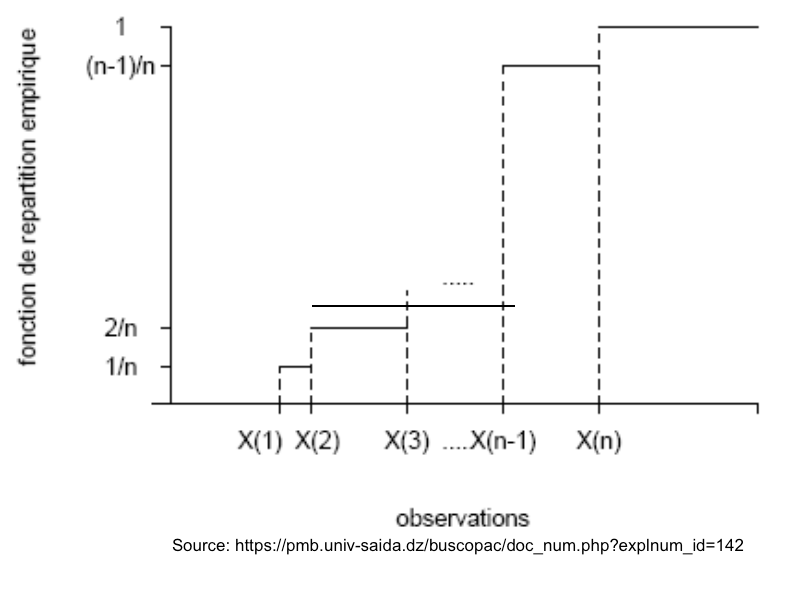
\includegraphics[scale=0.4]{Figures/Fct_repartition_empirique.png}
	\caption{Fonction de répartition empirique}
 \end{figure}
 \footnotemark{\url{https://pmb.univ-saida.dz/buscopac/doc_num.php?explnum_id=142}}

\paragraph{Remarques}
\begin{enumerate}[label=(\arabic*)]
\item Lorsque $F_n(t) \to F(t)$, alors

\item Puisqu'on a
\begin{align*}
\sum_{i=1}^{n} 1_{[x_i \leq t]} \sim Bin(n,\prob{X \leq t})
\end{align*}
Alors,
\begin{align*}
\esp{F_n(t)}		& = \frac{1}{n} n F(t) \\
	& = F(t) \quad \text{(C'est un estimateur sans biais)} \\
Var \left( F_n(t) \right) & = \frac{1}{n^2}  n F(t) S(t) \\
	& = \frac{F(t) S(t)}{n}	\\
	& \underset{n \to \infty}{=} 0 \\
\end{align*}
\end{enumerate}

\subsection{Estimation de donnée groupées (Fonction OGIVE)}
\red{\textbf{CETTE MATIÈRE NE SERA PAS TESTÉE À L'EXAMEN}}


%% VOIR SECTION 11.3 dans le livre %%
% Grahique de fonction de répartition empirique à insérer ici
Dans certains contextes, on a $n$ données qui sont groupées en intervalle. La fonction OGIVE permet d'interpoler entre 2 points $x_i$ et $_{i+1}$.
% Graphique des c^(i) et des intervalles n à insérer ici %%
\begin{align*}
c_{j-1} 	 \leq x  \leq c_j \\
F_n(c_{j-1})	 \leq F_n(x)	 \leq F_n(c_j) \\
\end{align*}


La formule est
\begin{equation}
\label{eq:repart-OGIVE}
F_n^{\text{OGIVE}}(x) = \frac{c_j - x}{c_j - c_{j-1}} F_n(c_j -1) + \frac{x - c_{j-1}}{c_j - c_{j-1}} F_n(c_j)
\end{equation}
\paragraph{Remarques}
\begin{enumerate}[label=(\arabic*)]
\item Si $x = c_{j-1}$,
\begin{align*}
F_n(c_{j-1}) = F_n^{\text{OGIVE}}(c_{j-1}) \\
\end{align*}
\item Si $x = c_j$,
\begin{align*}
F_n(c_j) = F_n^{\text{OGIVE}}(c_j)
\end{align*}
\end{enumerate}

\begin{exemple}[Exemple concret]
L'assureur a groupé $n=10$ données en intervalles.
\begin{center}
\begin{tikzpicture}[x = 1cm]
% Dessiner la ligne
\draw[black, |->, thick]
	(0,0) -- (5,0);
			
% Indiquer les intervalles
\foreach \t in 	{0, 1, 2, 3, 4}
{
	\draw[thick]
		(\t, 0) -- ++(0, 5pt)
			node[above] {\t};
} 	
\end{tikzpicture}
\end{center}
Alors,
\begin{align*}
F_n(t)	& = \frac{1}{n} \sum_{i=1}^{n} I[x_i \leq t] \\
F_n(1)	& = \frac{2}{10} \\
F_n(2)	& = \frac{5}{10} \\
F_n(3)	& = \frac{9}{10} \\
F_n(4)	& = \frac{10}{10} \\
		& = 1 \\
\end{align*}
% graphique à insérer avec les F_n ci-dessus %%
\end{exemple}

En dérivant \eqref{eq:repart-OGIVE}, on obtient
\begin{align*}
f_n(x) 	& = \derivee{x} F_x(x) \\
		& = \frac{1}{c_j - c_{j-1}} F_x(c_j) - \frac{1}{c_j - c_{j-1}} F_n(c_{j-1}) \\
		& = \frac{F_n(c_j) - F_n(c_{j-1})}{c_j - c_{j-1}} \\ \numberthis
\end{align*}

\section{Estimation de la fonction de survie}
Soit $S_n(t)$ la fonction de survie empirique. Alors,
\begin{align*}
S_n(t) 	& = 1 - F_n(t) \\
		& = \frac{n}{n} - \frac{1}{n} \sum_{i=1}^{n} \indic{x_i \leq t} \\ 
		& = \frac{1}{n} \sum_{i=1}^{n} \left( 1 - \indic{x_i \leq t} \right) \\
		& = \frac{1}{n} \sum_{i=1}^{n} \indic{x_i > t} \\
\end{align*}

\section{Estimateur  Kaplan-Meier}

\section{l'approche conditionnelle pour estimer $S(t)$}
% timeline à ajouter ici

\begin{align*}
S(t)		& = \frac{S(t_1)}{S(t_0)} \times \frac{S(t_2)}{S(t_1)} \times ... \times \frac{S(t)}{S(t_{i-1}} \\
	& = \frac{S(t)}{\underbrace{S(t_0)}_{1}} \\
	& = S(t) \\
\end{align*}
Alors,
\begin{equation}
S(t) = \prod_{j \leq t} \px{j}
\end{equation}
Ça nous suggère un autre estimateur pour $S(t)$ : 
\begin{equation}
\hat{S}(t) = \prod_{j \leq t} (1 - \hat{q}_j )
\end{equation}
Ceci est l'approche conditionnelle pour estimer $S(t)$. Et si jamais on a des données complètes, $S_n(t) = \hat{S}(t)$.




\end{document}
